\documentclass[11pt]{article}
\usepackage[T1]{fontenc}
\usepackage{lmodern}
\usepackage{amsmath,amssymb,amsthm,mathtools}
\usepackage[margin=1in]{geometry}
\usepackage{booktabs,array,longtable}
\usepackage{tikz}
\usetikzlibrary{positioning,fit}
\usepackage{listings}
\usepackage{microtype}
\usepackage[hidelinks]{hyperref}
\hypersetup{pdftitle={A sharp lower general-position bound for Cartesian products}}
\newtheorem{theorem}{Theorem}[section]
\newtheorem{lemma}[theorem]{Lemma}
\newtheorem{proposition}[theorem]{Proposition}
\newtheorem{corollary}[theorem]{Corollary}
\theoremstyle{definition}
\newtheorem{definition}[theorem]{Definition}
\theoremstyle{remark}
\newtheorem{remark}[theorem]{Remark}
\newcommand{\lgp}{\operatorname{gp}^{-}}
\newcommand{\MET}{\operatorname{MET}}
\newcommand{\supp}{\operatorname{supp}}
\newcommand{\GP}{\mathrm{GP}}
\newcommand{\card}[1]{\lvert #1\rvert}
\lstset{basicstyle=\ttfamily\small,columns=fullflexible,keepspaces=true,
  showstringspaces=false,breaklines=true,frame=single,rulecolor=\color{black!25}}

\title{A sharp lower general-position bound\protect\\for Cartesian products}
\author{Author information pending confirmation}
\date{Private working manuscript, version 0.1\quad 12 October 2026}

\begin{document}
\maketitle
\begin{abstract}
The lower general-position number of a finite graph is the smallest cardinality
of an inclusion-maximal vertex set containing no three vertices on a geodesic.
We refute the conjecture that the lower general-position number of a Cartesian
product is at least the smaller of the two factor parameters. For every integer
$r\geq 6$, we construct connected diameter-two factors of orders $2r-1$ and
$4r+5$ whose smaller factor parameter is $r$, while their product has lower
general-position number exactly five. Thus the conjectured bound can fail by
an arbitrarily large additive amount and an arbitrarily small ratio. We prove
the sharp replacement
$\lgp(G\square H)\geq\min\{5,\lgp(G),\lgp(H)\}$ for all nonempty finite
simple graphs. The lower bound has a computer-assisted proof reducing arbitrary
distances to equality patterns in the five-point pseudometric cone, followed
by an exact finite obstruction check. The construction and unbounded-gap
argument are elementary. An accompanying Lean proof verifies the fixed
$11$-by-$29$ counterexample at the level of actual shortest paths; it does
not formalize the universal bound.
\end{abstract}

\noindent\textbf{Keywords:} lower general position; Cartesian product;
graph distance; counterexample; metric cone; computer-assisted proof.

\noindent\textbf{MSC 2020:} 05C12, 05C69, 05C76.

\section{Introduction}

For a finite graph $G$, a general-position set contains no three distinct
vertices on any shortest path. Its lower general-position number $\lgp(G)$
minimizes cardinality over \emph{inclusion-maximal} general-position sets.
Unlike the ordinary general-position number, it measures the smallest terminal
outcome of adding vertices while maintaining general position. The parameter
was studied systematically by Di Stefano, Klav\v{z}ar, Krishnakumar, Tuite and
Yero~\cite{lowerGP}. Products expose a particular difficulty: maximality in a
factor need not translate into maximality in a product.

Kruft Welton, Khudairi and Tuite~\cite{WKT} proposed that
\begin{equation}\label{eq:original}
 \lgp(G\square H)\geq\min\{\lgp(G),\lgp(H)\}.
\end{equation}
This is Conjecture~3 on page~117 of their published paper and
Conjecture~2.10 in arXiv:2404.19451v1. We give connected counterexamples and
determine the best universal lower bound depending only on the smaller factor
parameter.

\begin{theorem}\label{thm:universal}
For all nonempty finite simple undirected graphs $G,H$,
\begin{equation}\label{eq:five}
 \lgp(G\square H)\geq\min\{5,\lgp(G),\lgp(H)\}.
\end{equation}
\end{theorem}

\begin{theorem}\label{thm:family}
For every integer $r\geq6$, there are connected diameter-two graphs $G_r,H_r$
with $\card{V(G_r)}=2r-1$ and $\card{V(H_r)}=4r+5$ such that
\[
 \lgp(G_r)=r,\qquad \lgp(H_r)\geq r,\qquad
 \lgp(G_r\square H_r)=5.
\]
The proof of the first two assertions and of the product upper bound $5$ is
elementary and does not use Theorem~\ref{thm:universal}.
\end{theorem}

\begin{corollary}\label{cor:optimal}
For each positive integer $r$, define
\[
 \Phi(r)=\min\bigl\{\lgp(G\square H): G,H\text{ are nonempty finite simple graphs},
 \ \min\{\lgp(G),\lgp(H)\}=r\bigr\}.
\]
Then $\Phi(r)=\min\{r,5\}$. In particular, \eqref{eq:original} holds whenever
one factor has lower general-position number at most five, but no unbounded
function of the smaller factor parameter is a universal product lower bound.
\end{corollary}

The five-point set in our construction uses three first-coordinate roles and
five second-coordinate roles. Large true-twin cliques increase the factor
parameters without changing the distance relations that block extensions in
the product. This separates factor saturation from product saturation and
explains the unbounded failure of \eqref{eq:original}.

The universal statement requires a different argument. A maximal product set
with fewer than five vertices would impose a finite collection of incompatible
factor-extension demands. Arbitrary factor distances are reduced to the zero
patterns of distances and triangle slacks in $\MET_5$. The finite obstruction
check uses integer arithmetic throughout. Its derivation, exhaustive-search
invariant and output are given in Sections~\ref{sec:metric}--\ref{sec:certificate}.

\subsection*{Relation to prior work}

The complete-factor formula is already known~\cite{WKT}. That paper's
unbounded-gap examples concern factor lower \emph{terminal} numbers,
rather than the factor lower general-position numbers used here.
We include the familiar complete-factor equality cases for sharpness.

True-twin saturation and clique enlargement are established tools; related
constructions appear in Bre\v{s}ar and Yero~\cite[Section~2.2,
Proposition~5]{BY}. We prove the required saturation lemma explicitly and
do not claim that general mechanism as new. The halfspace-clipping method
used below is standard polyhedral theory~\cite{Avis}. Our contribution is
the particular counterexample family, the sharp product bound and the
finite profile obstruction establishing that bound. Literature checks did
not locate a verified earlier solution with this scope; they do not certify
historical priority.

\section{Definitions and preliminary facts}\label{sec:definitions}

All graphs in this paper are finite, simple and undirected. A graph is
\emph{nonempty} when it has at least one vertex. A geodesic is a shortest path
between its endpoints. In a connected graph, distinct vertices $x,y,z$ are
collinear if one of
\[
 d(x,y)+d(y,z)=d(x,z),\quad
 d(x,z)+d(z,y)=d(x,y),\quad
 d(y,x)+d(x,z)=d(y,z)
\]
holds. A subset is in general position, or is a GP set, if it has no collinear
triple. This is equivalent to the shortest-path definition: a subpath of a
geodesic is geodesic, and a distance equality concatenates two geodesics to a
geodesic through the middle vertex. In disconnected graphs we use the
shortest-path definition, so vertices in different components cannot occur
on one path.

\begin{definition}
A GP set $S\subseteq V(G)$ is \emph{maximal} if it is inclusion-maximal:
$S\cup\{x\}$ fails to be GP for every $x\in V(G)\setminus S$. We set
\[
 \lgp(G)=\min\{\card S:S\subseteq V(G)\text{ is a maximal GP set}\}.
\]
\end{definition}
The minimum exists by finiteness. GP is hereditary, so failure of all
one-vertex extensions is equivalent to inclusion-maximality. Since $G$ is
nonempty, the empty set is never maximal and $\lgp(G)\geq1$.

The Cartesian product $G\square H$ has vertex set $V(G)\times V(H)$.
Two distinct vertices $(a,b),(a',b')$ are adjacent if either $a=a'$ and
$bb'\in E(H)$, or $b=b'$ and $aa'\in E(G)$.

\begin{lemma}\label{lem:distance}
For connected $G,H$,
\[
 d_{G\square H}((a,b),(a',b'))=d_G(a,a')+d_H(b,b').
\]
\end{lemma}
\begin{proof}
Every product path has at least $d_G(a,a')$ first-coordinate edge steps and
at least $d_H(b,b')$ second-coordinate edge steps. Conversely, concatenate
a first-coordinate geodesic with a second-coordinate geodesic.
\end{proof}

\begin{lemma}[True-twin saturation]\label{lem:twins}
Let $G$ be connected, and let $x,y$ be distinct vertices with $N[x]=N[y]$.
If a GP set contains $x$ and omits $y$, adjoining $y$ preserves general
position. Consequently, every maximal GP set meeting a true-twin clique
contains that entire clique.
\end{lemma}
\begin{proof}
The equality of closed neighborhoods implies $xy\in E(G)$. Interchanging
$x,y$ and fixing all other vertices is an automorphism, so
$d(x,w)=d(y,w)$ for $w\notin\{x,y\}$. A triple containing $y$ but not $x$
has the same distances as the corresponding triple with $x$. The distances
of a triple $x,y,w$ are $1,t,t$ with $t\geq1$, and none satisfies a triangle
equality. These are all new triples. Repeatedly apply this observation in
a true-twin clique.
\end{proof}

\begin{lemma}\label{lem:diameter-two}
In a connected graph of diameter at most two, a set is GP if and only if
its induced subgraph is a disjoint union of cliques.
\end{lemma}
\begin{proof}
A collinear triple must have distances $1,1,2$, so it is exactly an induced
three-vertex path. A graph contains no induced three-vertex path if and
only if each of its connected components is complete: a shortest path
between nonadjacent vertices in a noncomplete component supplies such a
triple.
\end{proof}

\section{An elementary counterexample family}\label{sec:construction}

Fix $r\geq6$. Let $A,B$ be disjoint cliques of order $r-1$ and adjoin a
vertex $c$ adjacent to every vertex of $A\cup B$, with no edges between
$A$ and $B$. Thus $G_r$ consists of two copies of $K_r$ intersecting only
in $c$. Choose $a\in A$ and $b\in B$.

For $H_r$, begin with
\[
 L=\{z,u_0,u_1,v_0,v_1\}.
\]
The subgraph induced by $L$ is $K_5$ with $u_0u_1$ and $v_0v_1$ deleted.
For each $i,j\in\{0,1\}$, add a clique $Q_{ij}$ of order $r$; its vertices
are adjacent outside $Q_{ij}$ precisely to $z,u_i,v_j$. There are no edges
between different $Q$-cliques. Equivalently,
$\{z,u_i,v_j\}\cup Q_{ij}$ is a complete graph for each $i,j$.
Both $c$ and $z$ are universal in their respective graphs. Nonadjacent
vertices exist in each factor, so both graphs have diameter two. Their
orders and edge counts are
\begin{equation}\label{eq:sizes}
 \begin{aligned}
 \card{V(G_r)}&=2r-1,&\quad \card{E(G_r)}&=r(r-1),\\
 \card{V(H_r)}&=4r+5,&\quad \card{E(H_r)}&=2r^2+10r+8.
 \end{aligned}
\end{equation}

\begin{figure}[htbp]
\centering
\begin{minipage}{.36\textwidth}
\centering
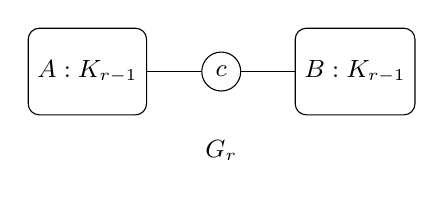
\begin{tikzpicture}[x=1cm,y=1cm,every node/.style={font=\small}]
 \node[draw,rounded corners,minimum width=1.25cm,minimum height=1.1cm] (A) at (-2.4,0) {$A:K_{r-1}$};
 \node[circle,draw,inner sep=3pt] (c) at (-.7,0) {$c$};
 \node[draw,rounded corners,minimum width=1.25cm,minimum height=1.1cm] (B) at (1,0) {$B:K_{r-1}$};
 \draw (A)--(c)--(B);
 \node at (-.7,-1) {$G_r$};
\end{tikzpicture}
\end{minipage}\hfill
\begin{minipage}{.59\textwidth}
\centering
$\displaystyle
 H_r=\bigcup_{i,j\in\{0,1\}}K_r[Q_{ij}]\vee K_3[\{z,u_i,v_j\}]$
\par\medskip
Four complete blocks, sharing\\only their indicated landmarks
\end{minipage}
\caption{Construction scheme. The two lines on the left indicate complete
adjacency from $c$ to the displayed cliques. On the right the union is a union
of graphs on the stated shared vertex sets; each individual joined block is
$K_{r+3}$. No edges are added between different $Q_{ij}$.}
\label{fig:scheme}
\end{figure}

\begin{proposition}\label{prop:factors}
The maximal GP sets of $G_r$ are $\{c\}\cup A$, $\{c\}\cup B$ and
$A\cup B$. Hence $\lgp(G_r)=r$. Moreover, $\lgp(H_r)\geq r$.
\end{proposition}
\begin{proof}
A GP set of $G_r$ containing $c$ cannot meet both $A$ and $B$, since
$a'-c-b'$ is geodesic whenever $a'\in A,b'\in B$. It lies in one of
the two $K_r$ blocks, and maximality then requires the entire block.
A GP set omitting $c$ and contained in one side can add $c$; it is not
maximal. The set $A\cup B$ is GP by Lemma~\ref{lem:diameter-two}, and
any of its proper subsets can add a missing vertex from that set.
These cases give the stated classification and minimum $r$.

Each $Q_{ij}$ is a true-twin clique. Lemma~\ref{lem:twins} implies that
any maximal GP set meeting it has cardinality at least $r$. Suppose
instead that a maximal GP set is contained in $L$. It must be maximal
within $L$ as well. The maximal GP subsets of $L$ are exactly
\begin{equation}\label{eq:landmark-sets}
 \{u_0,u_1\},\quad \{v_0,v_1\},\quad
 \{z,u_i,v_j\}\quad(i,j\in\{0,1\}).
\end{equation}
Indeed, a GP set containing $z$ must be a clique. A nonclique GP subset
of $L$ contains one of the two nonadjacent pairs, and any additional
landmark creates an induced three-vertex path. Any smaller clique can
be enlarged to one of the displayed triangles.

A vertex of $Q_{ij}$ extends $\{z,u_i,v_j\}$ to a clique. A vertex of
$Q_{00}$ extends either nonadjacent pair in \eqref{eq:landmark-sets},
since it is adjacent to exactly one vertex of that pair. Thus every
displayed set has an extension outside $L$, a contradiction. No
maximal GP set is contained in $L$, proving $\lgp(H_r)\geq r$.
\end{proof}

\begin{proposition}\label{prop:five-upper}
The set
\begin{equation}\label{eq:selected}
 S=\{s_0,s_1,s_2,s_3,s_4\}
   =\{(a,u_0),(a,u_1),(c,z),(b,v_0),(b,v_1)\}
\end{equation}
is a maximal GP set of $G_r\square H_r$. Consequently
$\lgp(G_r\square H_r)\leq5$.
\end{proposition}
\begin{proof}
Lemma~\ref{lem:distance} gives the selected distance matrix
\begin{equation}\label{eq:matrix}
 \begin{pmatrix}
 0&2&2&3&3\\2&0&2&3&3\\2&2&0&2&2\\
 3&3&2&0&2\\3&3&2&2&0
 \end{pmatrix}.
\end{equation}
The sum of two nonzero entries is at least four, larger than every
selected pair distance. Hence $S$ is GP.

Write $x=(g,h)\notin S$. Every $h\ne z$ is adjacent to $z$ and has
distance two from at least one of $u_0,u_1,v_0,v_1$: a landmark is
nonadjacent to its paired landmark, while a vertex of $Q_{ij}$ is
nonadjacent to $u_{1-i},v_{1-j}$.

If $g=c$, then $h\ne z$. Choose a selected point $s_t$ whose second
coordinate has distance two from $h$. We have
\[
 d(x,s_2)=1,\qquad d(s_2,s_t)=2,\qquad d(x,s_t)=3.
\]
Thus $s_2$ lies on an $x$--$s_t$ geodesic.

Suppose $g\in A$. If $h=z$, then
$d(x,s_2)=1$, $d(s_2,s_3)=2$ and $d(x,s_3)=3$.
If $h\notin\{z,u_0,u_1\}$, one of $v_0,v_1$ has distance two from
$h$: this is immediate for either $v$-landmark and for a $Q$-vertex.
With $t=3+j$ for such a $v_j$, we obtain
\[
 d(x,s_2)=2,\qquad d(s_2,s_t)=2,\qquad d(x,s_t)=4.
\]
Finally, if $h=u_i$, the fact that $x\notin S$ implies $g\ne a$, and
\[
 d(x,s_i)=1,\qquad d(s_i,s_{1-i})=2,\qquad d(x,s_{1-i})=3.
\]
Each subcase creates a collinear triple with two selected vertices.

For $g\in B$, apply the same argument under the graph symmetry exchanging
$A,B$, $a,b$, $u_i,v_i$ and $Q_{ij},Q_{ji}$. The first-coordinate
roles $c,A,B$ exhaust $V(G_r)$, so every outside vertex is blocked.
Thus $S$ is maximal.
\end{proof}

\begin{corollary}\label{cor:counterexample}
The conjecture \eqref{eq:original} is false even for connected factors of
diameter two. For the family above its additive deficit is at least $r-5$,
and the ratio of product lower general-position number to the smaller
factor parameter is at most $5/r$.
\end{corollary}
\begin{proof}
Combine Propositions~\ref{prop:factors} and~\ref{prop:five-upper}.
\end{proof}

\section{Reducing the universal bound to metric equality patterns}
\label{sec:metric}

We first assume that $G,H$ are connected. If Theorem~\ref{thm:universal}
fails, there is a maximal GP set
\[
 S=\{(a_i,b_i):0\leq i<k\},\qquad
 1\leq k\leq4,\quad k<\lgp(G),\lgp(H).
\]
The selected product vertices are distinct, but their coordinate projections
can repeat. The arrays
\[
 A_{ij}=d_G(a_i,a_j),\qquad B_{ij}=d_H(b_i,b_j)
\]
are therefore \emph{pseudometrics} on the $k$ labels: they are symmetric,
nonnegative and zero on the diagonal, and satisfy the triangle inequalities.
Zero distance identifies repeated actual vertices.

For three labels, a triangle equality holds in $A+B$ if and only if the
corresponding equality with the \emph{same middle label} holds in both $A$
and $B$. This follows because the two triangle slacks are nonnegative.
Likewise two product labels coincide if and only if their distance is zero
in both coordinates.

\subsection{Profiles and compatibility}

For a factor vertex $x$ and an unordered landmark pair $i<j$, record three
bits, in the order
\begin{equation}\label{eq:profile}
 \begin{split}
 d(a_i,x)+d(x,a_j)&=d(a_i,a_j),\\
 d(x,a_i)+d(a_i,a_j)&=d(x,a_j),\\
 d(x,a_j)+d(a_j,a_i)&=d(x,a_i).
 \end{split}
\end{equation}
Let $E(x)$ be the set of the $3\binom{k}{2}$ positions whose bits are true,
and let $Z(x)=\{i:d(x,a_i)=0\}$. We call $(E(x),Z(x))$ its profile.
Use the analogous definition for the second factor. For an outside factor
vertex $x\notin\{a_0,\ldots,a_{k-1}\}$, $Z(x)=\varnothing$.
Landmark vertices have their mandatory known profiles. Multiple bits in
\eqref{eq:profile} may be true when landmark coordinates repeat, and are
never replaced by a single mutually exclusive case.

\begin{lemma}\label{lem:compatibility}
If $S$ is GP, a factor-profile pair $(E,Z),(E',Z')$ corresponds to a
one-vertex GP extension of $S$ precisely when
\begin{equation}\label{eq:compatibility}
 Z\cap Z'=\varnothing,\qquad E\cap E'=\varnothing.
\end{equation}
Here the pair must be realized by actual factor vertices. We call any pair
of abstract profiles satisfying \eqref{eq:compatibility} \emph{compatible}.
\end{lemma}
\begin{proof}
The first condition says that the product point is not one of the selected
points. Since $S$ is GP, a new collinear triple must consist of that point
and two selected points. By distance additivity and nonnegative slacks,
it occurs exactly when both factors have an equality in the same one of
the three positions in \eqref{eq:profile}. This is excluded by the second
condition.
\end{proof}

\subsection{A complete finite cover of all distances}

Let $C=\MET_5\subseteq\mathbb R^{10}$ be the cone of all pseudometrics on
$\{0,1,2,3,4\}$, with coordinates $d_{ij}$ for $0\leq i<j\leq4$.
Its defining inequalities are the ten coordinate nonnegativities and the
thirty triangle inequalities
\begin{equation}\label{eq:cone}
 d_{ij}\geq0,\qquad d_{ij}+d_{j\ell}-d_{i\ell}\geq0
 \quad (i,j,\ell\text{ distinct}).
\end{equation}
Each of the three choices of middle label is used once for each unordered
triple. A pseudometric on the $k$ landmarks together with a new vertex
extends to $C$: put the new vertex at label $4$ and fill unused labels by
copies of label $0$. Thus this cone covers every distance pattern needed
for $k\leq4$, without bounding graph order, diameter or distances.

\begin{lemma}[Exact ray generation]\label{lem:rays}
The halfspace-clipping algorithm below enumerates all extreme rays of $C$,
using integer arithmetic. Its output has $25$ rays.
\end{lemma}
\begin{proof}
Begin with the ten unit rays of the nonnegative orthant and add the
triangle inequalities in lexicographic triple order. If the next
inequality is $h\geq0$, retain every old ray $r$ with $h(r)\geq0$.
For each adjacent old ray pair $r,s$ with $h(r)>0>h(s)$, add
\begin{equation}\label{eq:new-ray}
 h(r)s-h(s)r,
\end{equation}
normalized by the positive greatest common divisor of its coordinates.
The active inequalities of each ray are kept as a bit mask. Two distinct
old rays are adjacent exactly when no third old ray vanishes on all their
common active inequalities.

For completeness, every intermediate cone is pointed, since it lies in
the nonnegative orthant. It is full-dimensional, since the all-one vector
satisfies each coordinate and triangle inequality strictly. Intersecting
with $\sum_{i<j}d_{ij}=1$ gives a compact polytope. Clipping by a halfspace
retains the feasible old vertices and creates new vertices only on old
edges that cross its boundary. The minimal face containing two old
vertices is defined by their common active inequalities; it is an edge
if and only if it contains no third vertex. These observations justify
both the adjacency test and update~\eqref{eq:new-ray} inductively, starting
from the orthant. Every operation is exact rational, and the displayed
integer normalization avoids denominators. Running this update for the
thirty explicitly specified inequalities gives $25$ rays; the independent
replay derives them from \eqref{eq:cone}, rather than taking a ray table
as input. Its intermediate counts are given in
Appendix~\ref{app:certificate}.
\end{proof}

Let $\mathcal F$ be the forty nonnegative linear forms in
\eqref{eq:cone}. For $d\in C$, set
\[
 \mathcal Z(d)=\{f\in\mathcal F:f(d)=0\}.
\]

\begin{lemma}[Zero-pattern closure]\label{lem:closure}
All zero patterns $\mathcal Z(d)$ in $C$ are the intersections of subsets
of the $25$ extreme-ray zero patterns. The empty intersection is
$\mathcal F$, the pattern of the origin. There are $9484$ distinct patterns.
Each has an integer pseudometric representative.
\end{lemma}
\begin{proof}
Write $d=\sum_{r\in R}\lambda_r r$ for the extreme rays $R$ and
$\lambda_r\geq0$. Since each $f\in\mathcal F$ is nonnegative on every
ray, $f(d)=0$ if and only if $f(r)=0$ for every ray with $\lambda_r>0$.
Hence
\[
 \mathcal Z(d)=\bigcap_{\lambda_r>0}\mathcal Z(r).
\]
Conversely, the sum of the rays in any chosen subset realizes that
intersection; the empty subset gives the origin.
The checker starts with $\mathcal F$ and repeatedly intersects each
reached mask with each ray mask. A newly reached mask is stored with the
sum of the corresponding ray and the preceding representative, whose
forty zero tests are checked exactly. Queue exhaustion gives the entire
intersection closure, yielding $9484$ patterns. This enumerates
\emph{equality types}, not metrics up to a distance cutoff.
\end{proof}

\subsection{Landmark types and extension demands}

The \emph{landmark type} of a pseudometric records which landmark
distances are zero and which landmark triangle slacks are zero.
Group the patterns of Lemma~\ref{lem:closure} by their landmark type,
retaining patterns for which $d_{i4}>0$ for every $0\leq i<k$.
Every such pattern contributes an outside profile. Every actual outside
factor vertex is included, and all known profiles are determined by the
landmark type.

This step allows profiles having the same equality type but different
numerical landmark distances. It is a relaxation: the collected profiles
need not have a simultaneous realization in one graph. Nonexistence for
the relaxed system suffices, since it includes every actual factor system.

For a fixed landmark type, identify zero-distance labels and choose one
representative per distinct landmark. Let $T$ range over all maximal GP
subsets of these distinct landmarks. For each $T$ define its demand
\[
 \mathcal E_T=\{E:\ E\text{ is an outside profile and no bit for a pair in }T
 \text{ belongs to }E\}.
\]
The phrase ``a bit for a pair in $T$'' includes all three positions
in~\eqref{eq:profile} for that pair.

\begin{lemma}\label{lem:demands}
If a factor has lower general-position number larger than $k$, its set
$X$ of actual outside profiles intersects every $\mathcal E_T$.
\end{lemma}
\begin{proof}
The set $T$ has at most $k$ vertices, so it is not maximal in the entire
factor. It has an extending vertex. No distinct landmark can extend it,
by the choice of $T$. Thus the extending vertex is outside the landmark
set, and its profile has none of the prohibited pair bits.
\end{proof}

If $S$ were maximal, Lemma~\ref{lem:compatibility} would forbid compatible
pairs among all known and actual outside profiles. At the same time the
outside profiles on both sides would satisfy every demand of
Lemma~\ref{lem:demands}. The remainder of the connected-factor proof
excludes this finite system.

\section{Exact obstruction certificate and completion of the bound}
\label{sec:certificate}

\begin{proposition}[Finite obstruction]\label{prop:finite}
For each $k\in\{1,2,3,4\}$, no pair of landmark types can describe a GP
product set of size $k$ with outside-profile sets satisfying all demands
and avoiding every compatible pair, including pairs involving known
profiles.
\end{proposition}
\begin{proof}[Computer-assisted proof]
The data are generated by Lemmas~\ref{lem:rays} and~\ref{lem:closure}.
For every unordered pair of landmark types, reject pairs having a common
zero landmark distance or a common landmark triangle equality: they do
not describe distinct product vertices in general position. Factor
exchange makes unordered pairs sufficient.

If two known profiles are compatible, they already give a product
extension. Otherwise, let $A_G,A_H$ be the outside profiles remaining
after deleting all those compatible with a known profile on the opposite
side. Intersect each demand with its remaining profiles.

An exhaustive search selects second-factor profiles. Its state is
$(U,A)$, where $U$ is the set of unmet second-factor demands and $A$ is
the set of still permissible first-factor profiles. Initially every
second demand is unmet and $A=A_G$. If some first demand has empty
intersection with $A$, the state is impossible. Otherwise choose an
unmet second demand and branch over \emph{every} profile $q$ remaining
in it. Remove from $U$ all demands hit by $q$, and remove from $A$ all
profiles compatible with $q$. Repeated states may be merged.

If $U$ becomes empty while every first demand still meets $A$, choosing
all profiles in $A$ gives a feasible relaxed system. Indeed, profiles
within one factor have no additional compatibility requirement; only
cross-factor compatibility is relevant. The checker finds no such state.

This search is complete. Any hypothetical actual second-factor set
must contain a profile in the selected unmet demand and follows one of
the enumerated branches. All deleted first profiles are forbidden by
that selection. Each step meets a new second demand, so depth is finite.
Merging identical $(U,A)$ states is valid because future feasibility
depends only on these two objects. An empty demand has no branch and
is correctly rejected.

The exact output is shown in Table~\ref{tab:certificate}. The replay
scripts generate the cone, zero patterns, demands and search from their
definitions; no discovery table or solver output is read as proof input.
All four sizes return infeasibility for every surviving type pair.
\end{proof}

\begin{table}[htbp]
\centering
\begin{tabular}{rrrrr}
\toprule
$k$ & Landmark types & Outside profiles & GP type pairs & Search states\\
\midrule
1&1&1&1&2\\
2&2&5&2&3\\
3&8&87&14&15\\
4&106&9101&2381&2508\\
\bottomrule
\end{tabular}
\caption{Exact obstruction replay. The profile column is summed over all
landmark types. Known-profile obstructions can reject type pairs before
a search state is entered. The generator has $25$ rays and $9484$ zero
patterns in each run. The state totals include one additional state
from the demand-removal negative control in each run.}
\label{tab:certificate}
\end{table}

\begin{proof}[Proof of Theorem~\ref{thm:universal}]
For connected factors, a counterexample would give a maximal product GP
set of size $1\leq k\leq4$ with $k<\lgp(G),\lgp(H)$. Its actual
factor profiles satisfy the necessary demands and have no compatible
pair, contradicting Proposition~\ref{prop:finite}.

For disconnected factors, write their nonempty connected components as
$G_i$ and $H_j$. GP and maximality are componentwise, because a path
cannot connect different components. Therefore
\[
 \lgp(G)=\sum_i\lgp(G_i),\qquad
 \lgp(H)=\sum_j\lgp(H_j),
\]
and the components of the product are $G_i\square H_j$. Put
$x_i=\lgp(G_i)$ and $y_j=\lgp(H_j)$. The connected result gives
\[
 \lgp(G\square H)\geq\sum_{i,j}\min\{5,x_i,y_j\}.
\]
For nonnegative $t,y_j$, the elementary inequality
$\sum_j\min\{t,y_j\}\geq\min\{t,\sum_jy_j\}$ follows by considering
whether some summand reaches $t$. Apply it first with $t=\min\{5,x_i\}$
and then sum over $i$, to obtain
\[
 \sum_{i,j}\min\{5,x_i,y_j\}
 \geq\sum_i\min\{5,x_i,\textstyle\sum_jy_j\}
 \geq\min\{5,\textstyle\sum_ix_i,\sum_jy_j\}.
\]
This proves \eqref{eq:five} for all stated graphs.
\end{proof}

\begin{proof}[Proof of Theorem~\ref{thm:family} and Corollary~\ref{cor:optimal}]
For $r\geq6$, Theorem~\ref{thm:universal} supplies the lower bound five,
while Proposition~\ref{prop:five-upper} supplies the matching upper bound.
The factor parameters are given by Proposition~\ref{prop:factors}.

For $1\leq r\leq5$, take $G=H=K_r$, both with lower GP number $r$.
If a GP subset of $K_r\square K_r$ has cardinality less than $r$, an
unused first coordinate and an unused second coordinate give a point
at distance two from every selected point. It can be adjoined: selected
pair distances are at most two, whereas a new triangle has distances
$2,2,t$ with $1\leq t\leq2$. A full row is GP and maximal when $r\geq2$,
since every outside point is adjacent to the row point in its column,
which lies on a geodesic to any different row point. The case $r=1$
is the singleton graph. Thus the product has lower GP number $r$.
These equality examples and the universal bound show
$\Phi(r)=\min\{r,5\}$ for every positive integer $r$.
\end{proof}

\section{Formal verification and reproducible computation}
\label{sec:verification}

\subsection{The fixed original-conjecture counterexample}

Set $r=6$. Label the vertices of $G_6$ by $c=0$,
$a_i=1+i$ and $b_i=6+i$ for $0\leq i<5$. Label $H_6$ by
\[
 u_0=0,\quad u_1=1,\quad z=2,\quad v_0=3,\quad v_1=4,
 \quad Q_{ij}=\{5+6(2i+j),\ldots,10+6(2i+j)\}.
\]
The selected coordinate pairs are
$(1,0),(1,1),(0,2),(6,3),(6,4)$.
The factor orders are $11,29$, and their product has $319$ vertices.
Its edge count is
\[
 29\cdot30+11\cdot140=2410.
\]

The accompanying file \texttt{LowerGPProduct319.lean} defines actual finite
\texttt{SimpleGraph} factors and their Mathlib Cartesian product
\texttt{boxProd}. Its GP definition quantifies over actual shortest simple
\texttt{Walk}s and their vertex positions. The proof establishes equivalence
with the distance formulation, equivalence of one-point and inclusion
maximality, and the genuine minimum cardinality among maximal GP sets.
Its main fixed-object theorem proves
\[
 G_6,H_6,G_6\square H_6\text{ connected},\qquad
 \lgp(G_6)\geq6,\quad\lgp(H_6)\geq6,\quad
 \lgp(G_6\square H_6)\leq5.
\]
It also refutes the universal conjecture on the fixed finite vertex types
$11$ and $29$. These statements suffice to formalize the original
counterexample, without assuming a supplied distance table or the
universal-five theorem. The equality $\lgp(G_6)=6$ is proved above in
ordinary mathematics; it is not a separate audited equality endpoint in
this Lean file.

On 12 October 2026 the unchanged frozen source was compiled afresh with
Lean~4.34.1 and Mathlib commit
\texttt{d13f23b723b8a846827a245b89c10fc7d3f11612}, generating a new
\texttt{.olean} object. All fifteen audited declarations used only
\texttt{propext}, \texttt{Classical.choice} and \texttt{Quot.sound}; the
successful run had no error or warning. Full logs, source hashes, toolchain
identifiers and the fresh-object hash accompany the manuscript.
The all-parameter family, the universal bound and product equality five
are \emph{not} covered by this fixed-object Lean proof.

\subsection{Exact certificate replay}

The supplement contains three principal replay commands, using only the
Python standard library:
\begin{lstlisting}
python supplement/fixed319/verify.py
python supplement/universal/verify_universal_five.py
python supplement/universal/verify_unbounded_gap.py
\end{lstlisting}
The first reconstructs adjacency independently, computes all factor and
product BFS distances, compares factor BFS with Floyd--Warshall, and checks
all $319^2$ product distance entries against additivity. It verifies
all ten selected triples and actual shortest blocking paths for all
$314$ outside vertices. Factor subsets of cardinality at most five are
checked directly, along with the three maximal GP sets of $G_6$.

The second regenerates the metric rays, all equality masks and each of
the four obstruction problems in Table~\ref{tab:certificate}. The third
reconstructs the family at $r=6,7,12,31$ and checks the selected-distance
and blocking mechanisms, as well as the complete-factor equality cases
for $r=1,\ldots,5$. These finite regressions support the implementation;
the proof for every $r\geq6$ is Propositions~\ref{prop:factors}
and~\ref{prop:five-upper}, not extrapolation from those samples.

All three commands were executed successfully for this manuscript version.
Negative controls reject false maximality, a false GP extension, an
overstated factor lower bound and a genuine collinear factor triple.
The universal checker also removes the factor-extension demands: the
relaxed system then becomes feasible, as it should. It rejects a metric
violating an original triangle inequality and recognizes a collinear
three-point metric. These controls test meaningful failure modes; they
are not additional proofs of exhaustiveness.

\section{Discussion and scope}\label{sec:discussion}

The obstruction occurs because maximality is not preserved under
coordinate projection. In the family of Section~\ref{sec:construction},
true-twin saturation forces large maximal GP sets in $H_r$, but the product
can block every extension using only the five roles in \eqref{eq:selected}.
Increasing the clique sizes changes the factor parameters while leaving
that blocking mechanism intact. The metric certificate explains why the
same phenomenon cannot produce a maximal product GP set of size at most
four when both factor parameters are larger.

The sharpness is scalar: it determines the best bound from the smaller
factor lower-GP number alone. It does not give an exact formula for every
Cartesian product, classify all extremal pairs, minimize the order of a
counterexample, or resolve the separate terminal-set existence conjecture
in~\cite{WKT}. The construction establishes only the lower bound required
for $\lgp(H_r)$, without claiming its exact value for every $r$.

The universal proof has a finite computational component. Its mathematical
reduction is independent of distance cutoffs, and its checker uses exact
integer arithmetic with a complete search argument. Nevertheless, the
entire universal proof is not Lean formalized. A purely noncomputational
classification of the four-landmark obstruction would simplify this part
of the argument; the elementary original-conjecture counterexample does
not depend on such a classification.

\section*{AI assistance and manuscript status}

OpenAI Codex and a GPT-6-based agent system contributed substantially to
the mathematical construction, proof development, exact computation,
Lean formalization, literature searches, independent AI-agent checks and
manuscript writing. The independent AI reviewer of this manuscript did not
participate in discovering the construction or writing its proofs.
AI review and separate implementations do not constitute external human
peer review. No AI system is listed as an author. Human authorship,
contributions, responsibility review, funding and competing-interest
declarations, and the manuscript license remain to be confirmed before
public release. This working version is not a journal submission and has
no new DOI.

\appendix
\section{Replaying the finite obstruction}\label{app:certificate}

The halfspace order in \texttt{verify\_metric\_rays.py} takes unordered
triples $(a,b,c)$ lexicographically and, for each, the ordered triples
$(a,b,c),(a,c,b),(b,a,c)$, interpreted as outer--middle--outer labels.
Coordinates $d_{ij}$ use lexicographic unordered-pair order. The numbers of
extreme rays after the thirty successive triangle inequalities are
\[
\begin{gathered}
11,11,10,12,12,11,15,15,14,19,19,20,30,30,34,\\
49,49,64,58,52,46,42,34,30,26,22,22,23,24,25.
\end{gathered}
\]
The complete ray-to-zero-pattern generator and obstruction checker are
provided as executable source, without a third-party polyhedral or SAT
dependency. The essential search can be written as follows; all sets are
represented by bit masks in the implementation.

\begin{lstlisting}
check_pair(G, H):
    if a known-known profile pair is compatible:
        return INFEASIBLE
    A = G.outside_profiles incompatible with every H.known
    B = H.outside_profiles incompatible with every G.known
    D = [demand intersect B for demand in H.demands]
    stack = [(all demand indices, A)]
    seen = empty set
    while stack is not empty:
        (U, A) = pop(stack)
        if (U, A) is in seen: continue
        add (U, A) to seen
        if some G.demand has empty intersection with A: continue
        if U is empty: return FEASIBLE
        choose an unmet demand D[i]
        for every q in D[i]:
            Unew = U minus all demand indices hit by q
            Anew = A minus every profile compatible with q
            push (Unew, Anew)
    return INFEASIBLE
\end{lstlisting}

Neither exhaustion nor a digest alone supplies the semantic connection to
the original problem; that connection is proved by
Lemmas~\ref{lem:compatibility} and~\ref{lem:demands}. The exact code is
bound to this manuscript by \texttt{source-bindings.json}. Newly executed
outputs are in \texttt{verification/}; historical records in the source
supplement retain their original dates.

The four deterministic search-stream SHA256 digests, for $k=1,2,3,4$, are:
\begin{lstlisting}[basicstyle=\ttfamily\footnotesize]
96d806e0b6ceca36c5346273481079e390daa188fc97e4302f39b1dc0436133a
7772dbba1a8d4438b644d7b4fda05182389467038969c7629d5e9c239067d4e2
fa1fe74b732b9e524e0e13468067b8cb6651a50921f49632f025f4b5533c14ec
711f13a8995d9667bb276999ca636891a8ee82553193bbe068df0dc55ce1099f
\end{lstlisting}
These identify the replay streams under the fixed script version, not
historical priority or independent mathematical truth. The supplement's
manifest separately binds every included file by its SHA256 digest.

\section{Lean reproduction and provenance}\label{app:lean}

The Lean source digest is
\begin{lstlisting}[basicstyle=\ttfamily\footnotesize]
d1608a26b68eface444fc2c2feb53ebe8b24e364021213f589bd51e3aa52ab3e
\end{lstlisting}
Use Lean~4.34.1, the Mathlib revision specified in
Section~\ref{sec:verification}, and an existing cache or the ordinary
Mathlib cache-download procedure. From a Lake project with those pinned
dependencies, the source can be checked as
\begin{lstlisting}
lake env lean supplement/fixed319/LowerGPProduct319.lean
\end{lstlisting}
When checking a source outside that project's directory while producing
an object, pass \texttt{-R} with the source directory as the package root.
The supplied fresh-object receipt records the actual local command and
does not claim that an empty-cache machine was tested.

All mathematical inputs are bound to repository revision
\begin{lstlisting}[basicstyle=\ttfamily\footnotesize]
61488e05c9fe41984f483853f99e79f5715dc893
\end{lstlisting}
of \url{https://github.com/mio-qwq/math}. The construction originates in
the project's earlier frozen distributed result. Its construction and
the universal certificate are retained, respectively, at
\begin{lstlisting}[basicstyle=\ttfamily\footnotesize]
workstreams/ROOT/lower-gp-product319-counterexample/
workstreams/ROOT/distributed-written-proofs/B/lower_gp_product/
\end{lstlisting}
The manuscript gives the full mathematical argument rather than requiring
the reader to reconstruct it from development logs. Exact source provenance
and original version bindings accompany the supplement.

\begin{thebibliography}{9}
\raggedright

\bibitem{WKT}
E. Kruft Welton, S. Khudairi and J. Tuite,
\emph{Lower general position in Cartesian products},
Communications in Combinatorics and Optimization \textbf{10}(1) (2025), 110--125.
\href{https://doi.org/10.22049/cco.2024.29171.1879}{doi:10.22049/cco.2024.29171.1879}.
Preprint: \href{https://arxiv.org/abs/2404.19451v1}{arXiv:2404.19451v1}.

\bibitem{lowerGP}
G. Di Stefano, S. Klav\v{z}ar, A. Krishnakumar, J. Tuite and I. G. Yero,
\emph{Lower general position sets in graphs},
Discussiones Mathematicae Graph Theory \textbf{45} (2025), 509--531.
Preprint: \href{https://arxiv.org/abs/2306.09965}{arXiv:2306.09965}.

\bibitem{BY}
B. Bre\v{s}ar and I. G. Yero,
\emph{Lower (total) mutual-visibility number in graphs},
Applied Mathematics and Computation \textbf{465} (2024), 128411.
\href{https://doi.org/10.1016/j.amc.2023.128411}{doi:10.1016/j.amc.2023.128411}.
Preprint: \href{https://arxiv.org/abs/2307.02951v2}{arXiv:2307.02951v2}.

\bibitem{Avis}
D. Avis,
\emph{Excursions in Polyhedral Computation using lrs},
author-hosted mathematical exposition,
\url{https://cgm.cs.mcgill.ca/~avis/epc/epc.html}.
Accessed 12 October 2026.

\end{thebibliography}
\end{document}
